Proteins is the perhaps most important molecules of living
organisms. They perform a multitude of biological tasks and is found
in all lifeforms, from bacteria and unicellular organisms to
multicellular organisms such as animals. The chemical abilities and
biological functions of proteins is determined by their
three-dimensional structure. The ability to determine this structure
without performing costly experiments will have many applications in
medicine (e.g. drug design) and biotechnology. Protein structure
prediction and the related topic protein folding\footnote{The two
  research fields are distinguished by whether the actual folding
  process is simulated (protein folding) or a legal structure is
  sought without computing the intermediate steps (protein structure
  prediction).} are large and active research fields. It is still an
open problem.

\section{Protein structure}
The building blocks of proteins are amino acids\footnote{A detailed
  introduction to the structure of proteins is found in
  \cite{branden}}. There are twenty different amino acids which all
share a common structure. The type of amino acid is identified by an
attached molecule called the side-chain. A protein consists of one or
several unbranched chains (polymers) of amino acids. The order of
amino acids in such a chain is the primary structure of the protein.
The structure diagram in Figure \ref{fig:amino_connect} shows how a
sequence of amino acids are connected. The carbon atom connecting the
backbone with the side-chains is called the $C_\alpha$-atom. It is the
torsional angles around the two bonds connecting $C_\alpha$-atoms with
its neighbours ($N-C_\alpha$ and $C_\alpha-C'$), that contributes with
the highest variability to the determination of the protein structure
(see Section \ref{chap:protein_geometry}). Thus, when solving the
structure prediction problem it is common \fxwarning{cite} to cut down
the problem by using a model that describes the protein solely by its
$C_\alpha$-atoms. Such a sequence of $C_{\alpha}$ atoms is called a
$C_{\alpha}$-trace (see Figure \ref{fig:Calpha_backbone}). This is
also the representation used by the algorithms group at our department
and they therefore requested a method for subsequently adding the
remaining atoms to their model.

In Section \ref{chap:protein_geometry} we will describe the geometry
of the protein backbone and its side chains in detail.

%% Evt. Secondary structure: $\alpha$-helices, $\beta$-sheets
%% (+strands) and loops/turns.


\begin{figure}
  \centering
  \subbottom[]{
    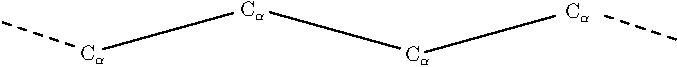
\includegraphics[width=0.48\textwidth]{figures/Calpha_backbone}  
    \label{fig:Calpha_backbone}
  }
  \subbottom[]{
    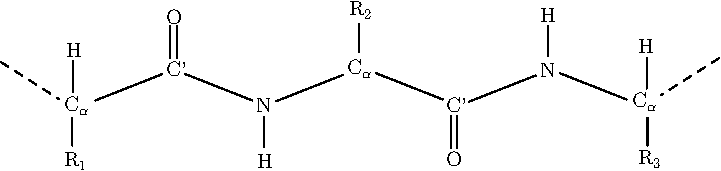
\includegraphics[width=0.48\textwidth]{figures/amino_connect}  
    \label{fig:amino_connect}
  }
  \caption{(a) $C_{\alpha}$-trace. (b) All-atom protein backbone, with $R_1$, $R_2$ and $R_3$ representing side-chains}
\end{figure}

\section{Protein structure prediction}
The chemical stability of a protein molecule is determined by the
amount of free energy in its structure. It is hypothesized
(\textit{Anfinsens dogma} or the \textit{thermodynamic hypothesis},
\cite{anfinsen73, soundararajan2010}) that all proteins has a unique
stable conformation where the free energy is minimized. This
conformation is known as the native structure of the
protein. Determining it computationally is the problem of protein
structure prediction. Thus, protein structure prediction is an energy
minimization problem.

% Why simplifications are necessary to make the problem
% computationally feasible.

There are generally two approaches to protein structure prediction.
\textit{Comparative modelling} uses information from known template
proteins with similar amino acid sequences while performing the
prediction. Another approach, called \textit{ab initio} or
\textit{de novo}, starts ``from scratch'' in the sense that no
information from known structures are used, but instead the
physical/chemical interactions between atoms forms the basis. This
\textit{ab initio} strategy is the approach taken by the algorithms
group at our department.

\subsection{Evaluating predictions}
%http://cnx.org/content/m11608/latest/
To determine the quality of prediction algorithms it is common \fxwarning{cite}
to compare predicted structures of a test proteins with the actual
known structure of that protein. The known structure of such test
proteins are obtained by other means (e.g. X-ray crystallography).
Thus a comparison measure between protein conformations are
needed. The most widely used comparison measure is \textit{least root mean
  square deviation}, lRMSD. RMSD is based on the distances between
corresponding atoms in the two protein conformations under comparison.
If $\vec{A}$ and $\vec{B}$ are two different conformations of the same protein,
where $\vec{a}_i$ and $\vec{b}_i$ are the respective coordinates of atom $i$ in the two
structures, RMSD can be computed by:
\begin{equation}
  \label{eq:rmsd}
  D(\vec{A}, \vec{B}) = \sqrt{\frac{1}{n}\sum_{i=1}^n |\vec{a}_i - \vec{b}_i|^2}
\end{equation}
To compute lRMSD, the RMSD has to be minimized by rotation and
translation of the two conformations. That is, to compute lRMSD, an
\textit{optimal superpositioning} of the conformations is found and
RMSD is computed.


% Limitation: A realistic energy calculation will require an insight in biochemistry
% that is beyond the scope of this project.  Therefore, we limit
% ourselves to minimize the number of clashes as well as the deviation
% from the provided $C_\alpha$-trace.


\section{Our strategy}
As mentioned, the algorithms group at our department uses a model that
only includes the the $C_\alpha$-atoms. Our goal with this project is
to extend this model with the remaining atoms to get an all-atom
model.  This will also enable the algorithms group to participate in
the CASP experiment \cite{caspwebsite}.

The strategy we will pursue, is to use a given $C_\alpha$-trace
generated by their prediction algorithm as target when fitting a
protein model that contains all atoms. The fitting should be conducted,
such that it minimizes the number of clashes and at the same time
minimizes the deviation from the target $C_\alpha$-trace.

We consider our fitting problem as two somewhat separate problems.
First, the backbone must be fitted to the \Ca-trace, only minimizing
the deviation to the $C_{\alpha}$-trace.  Hereafter, the amino acid
residues (side chains) are added to the backbone changing the backbone
conformation only if necessary.  In the following we have chosen to
consider these two tasks separately even though the residue handling
will cause changes in the backbone.

In Section \ref{chap:fitting_backbone}, we will describe the strategy we use to fit the all-atom backbone to the \Ca-trace ignoring the amino acid residues.
In Section \ref{chap:handling_sidechains}, we will explain how we add the side-chains to the all-atom backbone changing the backbone-conformation only if necessary.

%%% Local Variables: 
%%% mode: latex
%%% TeX-master: "rapport"
%%% End: 
